\begin{surferPage}[Quintic (15 Cusps)]{Une Quintique à 15 Pointes}
  Cette surface de degré $5$ (quintique) a $15$ singularités de type $A_2$
    (appelées pointes); cette quintique ainsi qu'une série associée de surfaces
    a été introduite par Oliver Labs dans un article de 2005.
    Cinq pointes se distinguent particulièrement des autres.
    En fait, ce sont cinq singularités de type $A_2^{++}$, les dix autres sont de type $A_2^{+-}$ (voir
    la galerie sur les singularités simples pour plus de détails) :

     \vspace*{-0.3em}
    \begin{center}
      \begin{tabular}{c@{\qquad}c}
        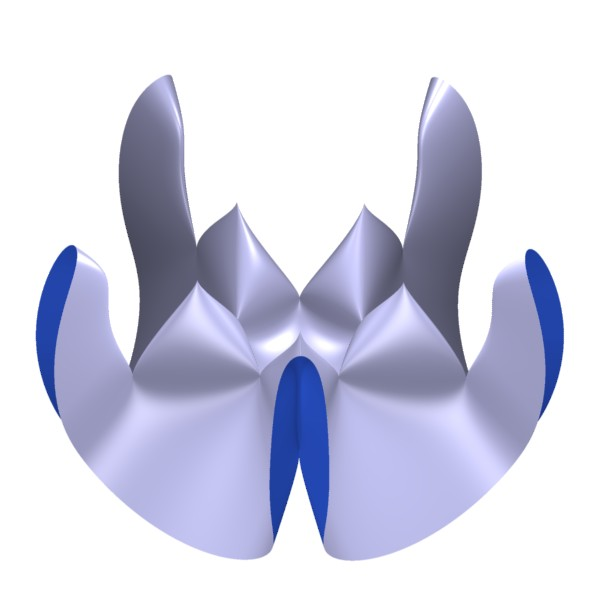
\includegraphics[height=1.2cm]{./../../common/images/dessins_quint_15a2}
        &
        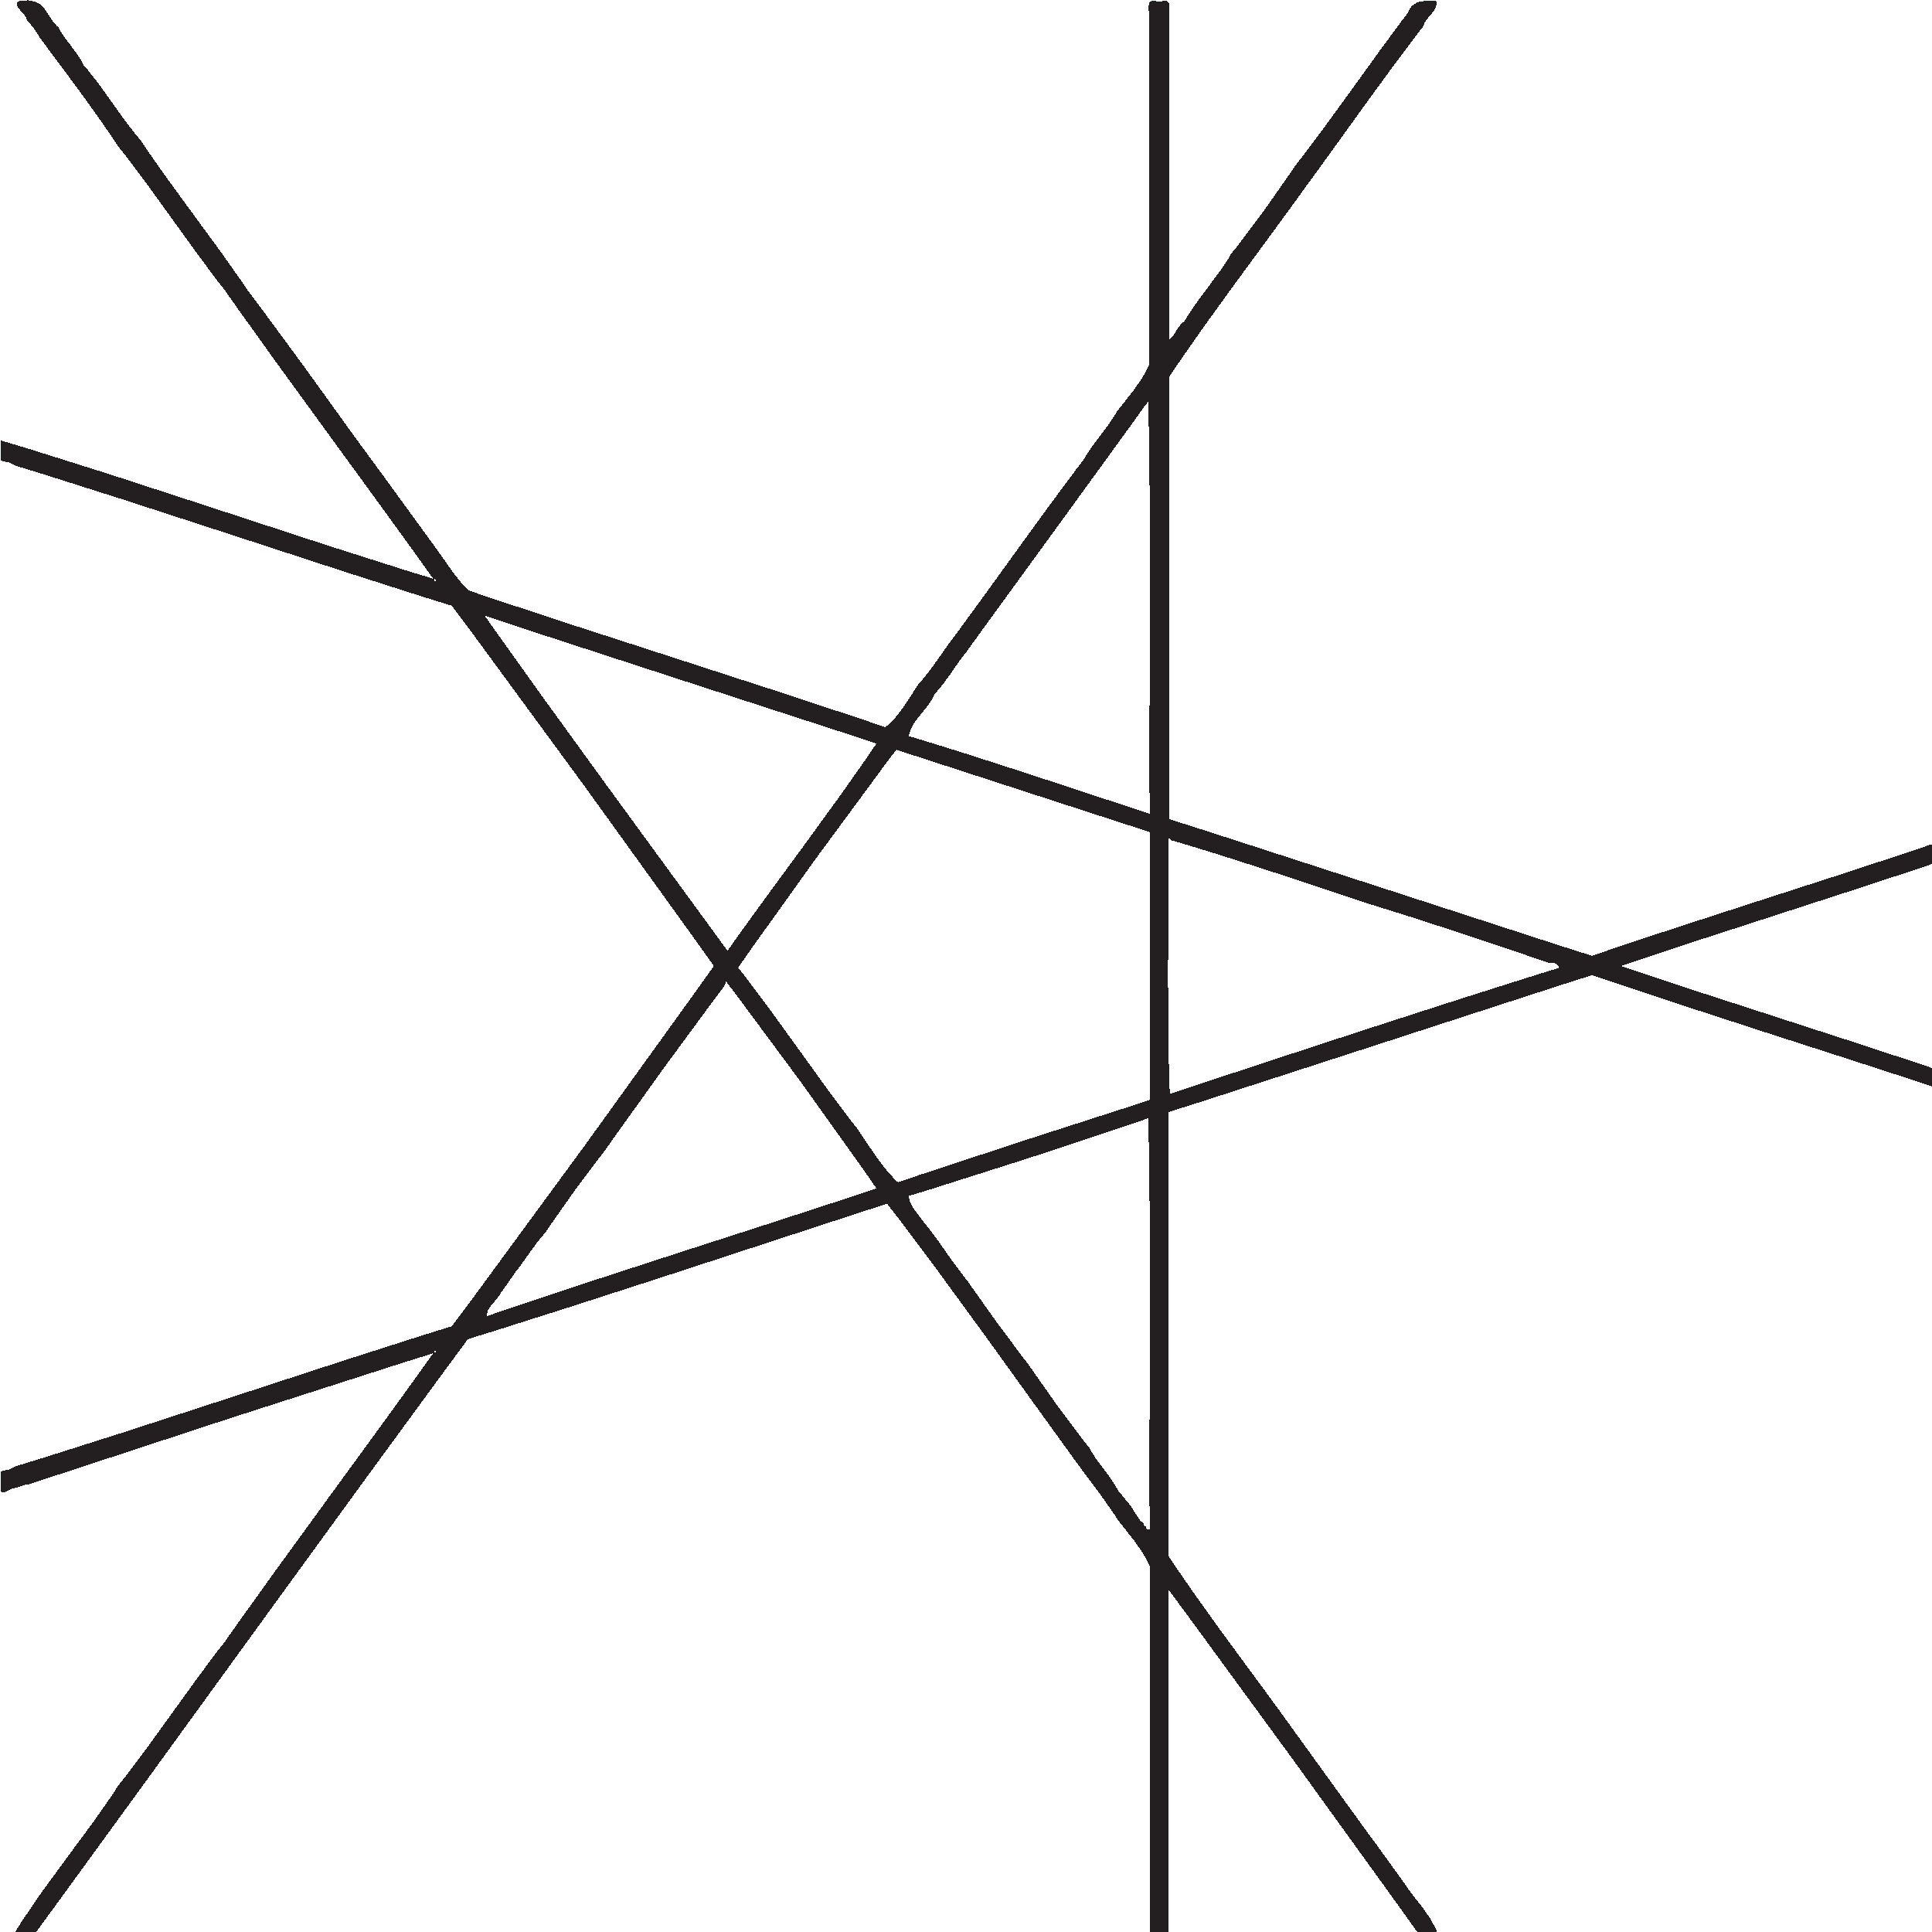
\includegraphics[height=1.2cm]{./../../common/images/rp5.pdf}
      \end{tabular}
    \end{center}
    \vspace*{-0.3em}    
    
    Cette surface a une équation de la forme 
    $S_5(x,y) + t(z)=0,$
    où $S_5(x,y)$ est un pentagone régulier (image de droite) et $t(z)$ est une
    variante des polynômes de Tchebychev déjà rencontrés à plusieurs
    reprises.

     Une autre quintique (à gauche) à $15$ pointes fut construite par
    Wolf Barth; elle est reliée à la Cubique de Clebsch (à droite) comme le montre l'image du
    milieu :

    \vspace*{-0.3em}
    \begin{center}
      \begin{tabular}{c@{\quad}c@{\quad}c}
        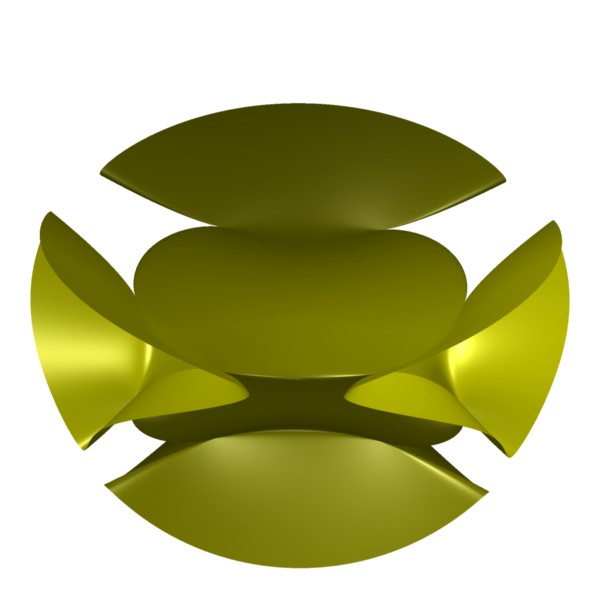
\includegraphics[height=1.2cm]{./../../common/images/barthquintic_green}
        &
        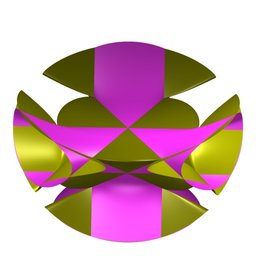
\includegraphics[height=1.2cm]{./../../common/images/barthquintic_clebschcubic}
        &
        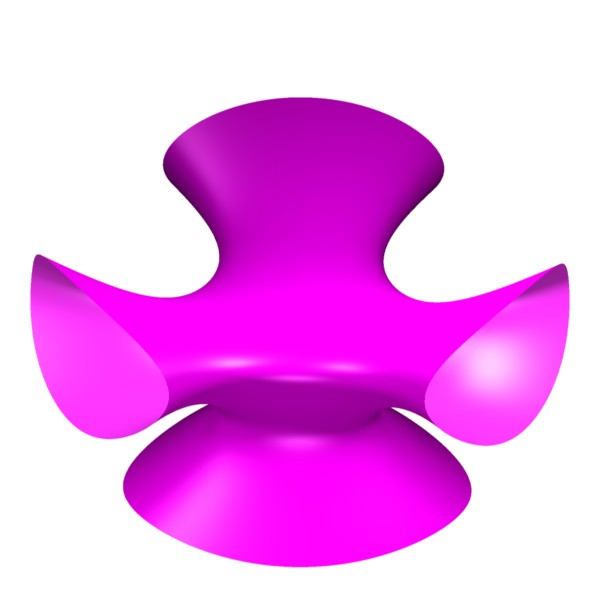
\includegraphics[height=1.2cm]{./../../common/images/clebschcubic_pink}
      \end{tabular}
    \end{center}
    \vspace*{-0.3em}
\end{surferPage}
